%TC:macro \todo [option:0,0]
\documentclass[12pt]{article}

\usepackage[utf8]{inputenc}
\usepackage[T1]{fontenc}
\usepackage[margin=1in]{geometry}
\usepackage{setspace}
\usepackage{hyperref}
\usepackage{titlesec}
\usepackage{mathptmx} % Times Roman font
\usepackage{amsmath}  % for \text command in math mode
\usepackage{graphicx}
\usepackage{wrapfig}
\usepackage[font=small,labelfont=bf]{caption}
\usepackage[numbers,sort&compress]{natbib}
\usepackage[disable,textsize=footnotesize,color=yellow!40]{todonotes}
\usepackage{catchfile}

% Automatic word count via texcount (run by latexmk; no -shell-escape needed).
% Counts body text only; excludes title block, captions, todos, and references.
\newcommand{\wordcount}{%
  \IfFileExists{\jobname.wordcount}%
    {\CatchFileDef{\thewordcount}{\jobname.wordcount}{\endlinechar=-1}%
     \thewordcount}%
    {[word count unavailable]}%
}

% Compact section formatting to maximize space
\titleformat{\section}{\normalfont\bfseries\large}{\thesection.}{0.5em}{}
\titleformat{\subsection}{\normalfont\bfseries\normalsize}{\thesubsection.}{0.5em}{}
\titlespacing*{\section}{0pt}{1.5ex plus 0.5ex minus 0.2ex}{0.8ex plus 0.2ex}
\titlespacing*{\subsection}{0pt}{1.0ex plus 0.3ex minus 0.2ex}{0.5ex plus 0.1ex}

% No page numbers on first page, numbers on subsequent pages
\pagestyle{plain}

\begin{document}

%TC:ignore
\begin{center}
{\large \textbf{Development of a Pitzer Ion-Interaction Framework for Predicting Sulfide-Mineral Precipitation in Produced-Water Brines}}\\[0.3em]
{\small Sterling G. Baird, Department of Mechanical Engineering, Brigham Young University}
\end{center}
%TC:endignore

\doublespacing

\section{Introduction}

\begin{wrapfigure}{r}{0.45\textwidth}
\centering
\vspace{-1.5em}
\includegraphics[width=0.4\textwidth]{../grants/acs-prf/figures/workflow-diagrams/proposal_overview_figure.png}
\caption{Overview of the proposed prediction framework. A high-throughput experimental platform generates Latin hypercube--sampled compositions of metal ions, sulfide, and brine matrix in 96-well plates. Precipitation is detected off-line via visual scoring, camera imaging, or microplate-reader absorbance, and results are compared to Pitzer-model predictions to identify deviations and regress new interaction parameters.}
\label{fig:overview}
\vspace{-1em}
\end{wrapfigure}

\todo[inline]{Add preliminary results before submission: (1)~a BaSO\textsubscript{4} precipitation experiment in a 96-well plate to demonstrate the OT-2 workflow (include photograph/image) and (2)~ideally a pilot FeS or PbS precipitation experiment showing visible precipitate formation. Replace placeholder figure boxes with real figures/data. (Note: the computational Pitzer gap analysis figure has been added as Figure~\ref{fig:phreeqc_si}.)}

Mineral scale formation is one of the most persistent operational challenges in petroleum production \cite{kan2019,jordan2000,crabtree1999}. When incompatible waters mix during extraction, dissolved metal ions precipitate as insoluble scales that restrict flow, foul equipment, and compromise well integrity \cite{kan2019,jordan2000}. Among the most problematic scales are barite (BaSO$_4$), iron sulfide (FeS, mackinawite), and lead sulfide (PbS, galena), all of which form readily from the metal ions and anions present in petroleum-produced waters \cite{wylde2014,alharbi2017}.

The thermodynamic framework used to predict scale formation in high-salinity brines is the Pitzer ion-interaction model, which accounts for non-ideal behavior through empirically determined interaction parameters \cite{kan2019}. For sulfate scales---particularly barite---Pitzer models are well-validated and predict saturation indices to approximately $\pm$0.1~SI in brines with total dissolved solids (TDS) exceeding 200,000~mg/L \cite{kan2019,shaferpeltier2020}. However, for sulfide scales (FeS and PbS), the situation is markedly different. Published solubility products for mackinawite vary by orders of magnitude, iron--sulfide speciation is complicated by complexes such as FeHS$^+$, and the practical pH threshold for FeS precipitation ($\sim$6.5) depends on brine composition in ways that current models do not fully capture \cite{wylde2014,wang2020}. For PbS, the mineral is effectively insoluble ($K_{\text{sp}} \approx 10^{-29}$), yet its solubility increases with both temperature and salinity in real brines. Duan et al.\ (2007) showed that galena solubility predictions in NaCl brines require approximations for missing Pb$^{2+}$--H$_2$S parameters and exhibit $>$15\% errors in CaCl$_2$ solutions \cite{duan2007}. Pitzer interaction parameters for Pb$^{2+}$--HS$^-$ in the presence of major brine cations have not been systematically validated \cite{alharbi2017,keogh2019}.

A critical gap exists: the higher-order mixing parameters ($\theta_{ij}$ and $\psi_{ijk}$) required by the Pitzer formalism for Fe$^{2+}$ and Pb$^{2+}$ with major produced-water ions (Na$^+$, Ca$^{2+}$, Cl$^-$) are sparse or absent from standard thermodynamic databases \cite{wang2020}. Models used in petroleum engineering therefore rely on parameters derived from simple binary or ternary electrolyte systems, yet produced waters routinely contain five to ten or more major dissolved species simultaneously \cite{kan2019,shaferpeltier2020}. Whether---and where---this simplification breaks down remains an open question.

This proposal develops a new Pitzer-based prediction framework for sulfide-mineral precipitation in complex brines by systematically determining the 34 unmeasured ion-interaction parameters through high-throughput experimentation across produced-water-relevant conditions. The fundamental question is: \textit{What are the binary, mixing, and neutral-species interaction parameters required to extend Pitzer theory to sulfide systems in multi-component brines, and how do these parameters govern precipitation boundaries at high ionic strength?}

\section{Objectives and Specific Aims}

The overarching objective of this project is to develop a complete Pitzer ion-interaction framework for predicting sulfide-mineral precipitation in multi-component brines by determining the 34 currently unmeasured binary, mixing, and neutral-species interaction parameters. We will accomplish this by generating the first comprehensive, systematically controlled experimental dataset of FeS and PbS precipitation boundaries, benchmarking current predictions, and regressing the missing parameters. We hypothesize that \textbf{existing Pitzer-model predictions for FeS and PbS precipitation boundaries will systematically deviate from experimental observations in multi-component brines at ionic strengths above $\sim$2~molal, because (1)~binary interaction parameters ($\beta^{(0)}$, $\beta^{(1)}$, $C^\phi$) for the Fe$^{2+}$--HS$^-$ and Pb$^{2+}$--HS$^-$ pairs are absent from standard databases, (2)~higher-order mixing parameters ($\theta_{ij}$ and $\psi_{ijk}$) for these cations with Na$^+$ and Ca$^{2+}$ have not been determined in sulfide media, (3)~neutral-species interaction parameters ($\lambda$, $\zeta$) for aqueous complexes such as FeS$^0_{\text{aq}}$ are unknown, and (4)~aqueous metal--sulfide and metal--chloride complexation must be coupled with activity-coefficient corrections to avoid compensating errors. Including temperature-dependent coefficients, metal--chloride terms, Pb$^{2+}$--SO$_4^{2-}$ binary parameters, and neutral-species parameters for PbCl$_2^0$, the full parameter set comprises 34 unknowns (see Aim~2). The Pb$^{2+}$ system, for which no Pitzer parameters of any kind exist for sulfide interactions \cite{wang2020,felmy2000}, represents the most critical gap.}

\subsection{Aim 1: Map Experimental FeS and PbS Precipitation Boundaries Across Produced-Water-Relevant Parameter Space}

We will systematically vary metal-ion concentration ([Fe$^{2+}$] and [Pb$^{2+}$]), sulfide concentration ([HS$^-$]), ionic strength (0.5--5~molal NaCl $\pm$ CaCl$_2$), pH (4--9), and temperature (25--90~$^\circ$C) in 96-well microplates using a Latin hypercube sampling design and an automated platform. Following automated plate preparation (the most labor-intensive step), precipitation is then detected via visual scoring of images and microplate-reader absorbance. The deliverable is a curated dataset of approximately 30,000 individual measurements ($\sim$5,000 unique conditions $\times$ triplicates per metal system), combining initial space-filling sampling with adaptive Bayesian-optimization-guided follow-up (see below).

\subsection{Aim 2: Quantify Deviations Between Experimental Boundaries and Pitzer-Model Predictions, and Regress New Interaction Parameters}

For each experimental condition, we will compute saturation indices using PHREEQC (free, open-source; USGS) with published Pitzer databases and compare predictions to observed precipitation boundaries. Where systematic deviations exceed $\pm$0.2~SI, new Pitzer interaction parameters---binary, mixing, neutral-species, and temperature-dependent terms (34 total; see below)---will be regressed using weighted least-squares fitting. The resulting parameters will be validated against held-out experimental conditions. The deliverable is a set of validated Pitzer interaction parameters for the Fe$^{2+}$--HS$^-$ and Pb$^{2+}$--HS$^-$ systems in NaCl--CaCl$_2$ brines, suitable for incorporation into standard thermodynamic databases such as the PHREEQC \texttt{pitzer.dat} database (USGS), the gebo extended Pitzer database \cite{bozau2013}, the Thermoddem database (BRGM), and ScaleSoftPitzer (Rice University).

\section{Background and Significance}

\subsection{Sulfide Scales in Petroleum Production}

Sulfide-scale deposition is a growing concern in petroleum production, particularly as reservoir souring introduces H$_2$S into formation and produced waters \cite{wylde2014,alharbi2017}. Iron sulfide (FeS) deposits are especially common in wells with even milligram-per-liter levels of dissolved iron, where the practical precipitation threshold occurs near pH~6.5 \cite{wylde2014}. Lead sulfide (PbS) is a major scale component in high-temperature North Sea reservoirs and other formations where lead concentrations reach tens of milligrams per liter \cite{alharbi2017,keogh2019}. Unlike sulfate scales, sulfide scales are often poorly predicted by existing models, leading to unexpected deposition and costly remediation \cite{wang2020}.

The economic impact is substantial. Scale-related production losses, chemical treatment costs, and intervention expenses account for billions of dollars annually across the petroleum industry; Hamza et al.\ (2021) estimated inorganic scale costs at \$1.4~billion per year, with individual well-intervention costs reaching \$2.5~million \cite{crabtree1999,kelland2014,hamza2021}. Accurate prediction of sulfide-scale formation would enable preventive chemical treatment programs, optimized water management, and reduced unplanned downtime \cite{kan2019,crabtree1999}.

\subsection{Pitzer Activity-Coefficient Models and Their Limitations}

The Pitzer formalism extends the Debye--H\"uckel theory to concentrated electrolyte solutions by including binary ($\beta^{(0)}$, $\beta^{(1)}$, $C^\phi$) and ternary ($\theta$, $\psi$) ion-interaction parameters \cite{kan2019}. For BaSO$_4$, these parameters have been extensively measured in NaCl, CaCl$_2$, and mixed brines, and Pitzer models predict barite saturation indices with high accuracy even at ionic strengths of 5--6~molal \cite{kan2019,shaferpeltier2020}. This success has made Pitzer-based codes (e.g., PHREEQC, ScaleSoftPitzer) the standard tools for scale prediction in petroleum engineering.

However, for sulfide minerals, the parameter database is far less complete. The USGS PHREEQC \texttt{pitzer.dat} database contains binary Pitzer parameters for Fe$^{2+}$ with only Cl$^-$ and SO$_4^{2-}$---no Fe$^{2+}$--HS$^-$ or Fe$^{2+}$--S$^{2-}$ parameters---and contains \textit{zero} Pitzer parameters for Pb$^{2+}$ with any anion \cite{wang2020}. Binary ($\beta^{(0)}$, $\beta^{(1)}$, $C^\phi$) and mixing ($\theta$, $\psi$) parameters for Fe$^{2+}$--HS$^-$ and Pb$^{2+}$--HS$^-$ are likewise absent from Thermoddem and other standard databases, even though HS$^-$ parameters with major cations are available \cite{millero1986} and Pb$^{2+}$--Cl$^-$ brine parameters have been measured \cite{felmy2000}. Notably, Bozau (2013) developed the ``gebo'' extended \texttt{pitzer.dat} database, adding master species for Fe, Pb, S($-$2), and other elements to enable process modeling in highly saline waters; however, Bozau explicitly noted that no literature Pitzer parameters could be found for Pb or Zn interactions with major ions, and the metal--sulfide Pitzer coefficients required for predictive modeling remain absent from the gebo extension \cite{bozau2013}. Similarly, the widely cited Pitzer database extension by Appelo (2015)---which provides high-temperature, high-pressure parameters for the Na--K--Mg--Ca--Ba--Cl--CO$_2$--HCO$_3$--SO$_4$--H$_4$SiO$_4$ system---does not include Fe$^{2+}$, Pb$^{2+}$, or any metal--sulfide Pitzer parameters \cite{appelo2015}.

Published mackinawite $K_{\text{sp}}$ values range from $10^{-3.6}$ to $10^{-4.65}$ \cite{wylde2014,wang2020}, and above pH~6, stable aqueous complexes and nanoparticulate precursors further complicate thermodynamic analysis \cite{kan2019}. Wang et al.\ (2020) noted that models fall back on Debye--H\"uckel or Davies-equation estimates for sulfide systems at high ionic strength \cite{wang2020}. For PbS, Felmy et al.\ (2000) developed a Pitzer model for Pb$^{2+}$ in chloride--sulfate brines but found that predictions fail above $I \approx 2$~molal \cite{felmy2000}; crucially, their model does not include sulfide interactions. Al-Harbi et al.\ (2017) showed that PbS precipitation is rapid and nearly stoichiometric until Pb:S$\approx$1, but did not systematically explore brine matrix effects \cite{alharbi2017}.

Critically, neither the binary parameters ($\beta^{(0)}$, $\beta^{(1)}$, $C^\phi$) for Fe$^{2+}$--HS$^-$ and Pb$^{2+}$--HS$^-$, nor the higher-order mixing parameters ($\theta$, $\psi$) for these cations with Na$^+$ and Ca$^{2+}$, have been determined for sulfide systems in complex brines. This amounts to 34 unmeasured parameters when neutral-species interactions, temperature-dependent coefficients, Pb$^{2+}$--SO$_4^{2-}$ binary terms, and PbCl$_2^0$ neutral-species interactions are included (see Aim~2 for a full enumeration). The persistence of this gap across multiple independent database-extension efforts---Bozau's gebo dataset \cite{bozau2013} and Appelo's high-temperature extension \cite{appelo2015}---underscores that the missing metal--sulfide Pitzer parameters represent a fundamental data gap that cannot be resolved by database compilation alone but requires new experimental measurements. Our own PHREEQC computations confirm this gap: whereas barite SI predictions remain smooth and well-behaved across $I = 0.1$--5~molal using the Pitzer database, mackinawite SI can only be computed with the Davies equation (\texttt{phreeqc.dat}), which is unreliable above $I \approx 0.5$~molal. Furthermore, adequate modeling requires coupling Pitzer-framework calculations with comprehensive aqueous speciation, including metal--chloride and metal--sulfide complexation \cite{kan2019,felmy2000}; neglecting this coupling likely contributes as much to model inaccuracy as missing mixing parameters.

\subsection{Automated High-Throughput Precipitation Screening}

The Latin hypercube sampling (LHS) experimental design required to systematically probe precipitation boundaries across multiple variables (metal concentration, sulfide concentration, ionic strength, pH, temperature) generates hundreds of conditions per experiment. Manual execution of such matrices is prohibitively time-consuming and subject to inconsistency.

Automated high-throughput experimental platforms address this limitation. Robotic nephelometry in 96-well microplates has been validated for kinetic solubility determination in pharmaceutical contexts, where Dehring et al.\ (2004) demonstrated that automated turbidity measurements reliably detect precipitation onset \cite{dehring2004}. Petru\v{s}evska et al.\ (2013) showed that matrix-matched blanks enable accurate turbidity-based precipitation detection even in complex backgrounds \cite{petrusevska2013}. In materials science, Velasco et al.\ (2021) used an Opentrons OT-2 to automate high-throughput co-precipitation of multicomponent oxide libraries in 96-well plates, processing over 100 samples per day \cite{velasco2021}; this methodology has since been extended by the same group for high-throughput screening of high-entropy fluorite oxides \cite{kumbhakar2023} and paired with automated XRD phase identification \cite{schuetzke2023}, confirming the OT-2's suitability for systematic inorganic phase-space exploration. However, none of these citing works address aqueous mineral scale precipitation---the current state of practice in oilfield scale evaluation relies on low-throughput NACE static bottle tests or kinetic turbidity assays with $\sim$12~simultaneous samples \cite{baugh2012}. This creates an opportunity to bring high-throughput screening methodologies to a petroleum-relevant inorganic chemistry problem.

\textbf{Safety and environmental controls.} All experiments involving sulfide solutions will be conducted with the OT-2 housed inside a chemical fume hood to contain H$_2$S off-gassing. Chemically resistant polypropylene well plates and filter-tipped pipette tips will be used to prevent cross-contamination and protect the sample-preparation hardware from corrosive solutions. Environmental monitoring within the enclosure will include continuous humidity and ambient temperature logging, as well as H$_2$S gas detection to ensure concentrations remain below permissible exposure limits. For the elevated-temperature subset (60--90~$^\circ$C), experiments will be conducted in sealed glass vials rather than open microplate wells to minimize H$_2$S partitioning into the headspace, which is significant at pH~$<$~6 and high temperature; control experiments with alternating high-sulfide and blank wells will quantify any cross-well H$_2$S diffusion. These controls ensure safe handling of sulfide-bearing solutions and reliable, reproducible experimental conditions.

\section{Research Plan}

\subsection{Aim 1: Experimental Precipitation Boundary Mapping}

\begin{wrapfigure}{r}{0.4\textwidth}
\centering
\vspace{-1.5em}
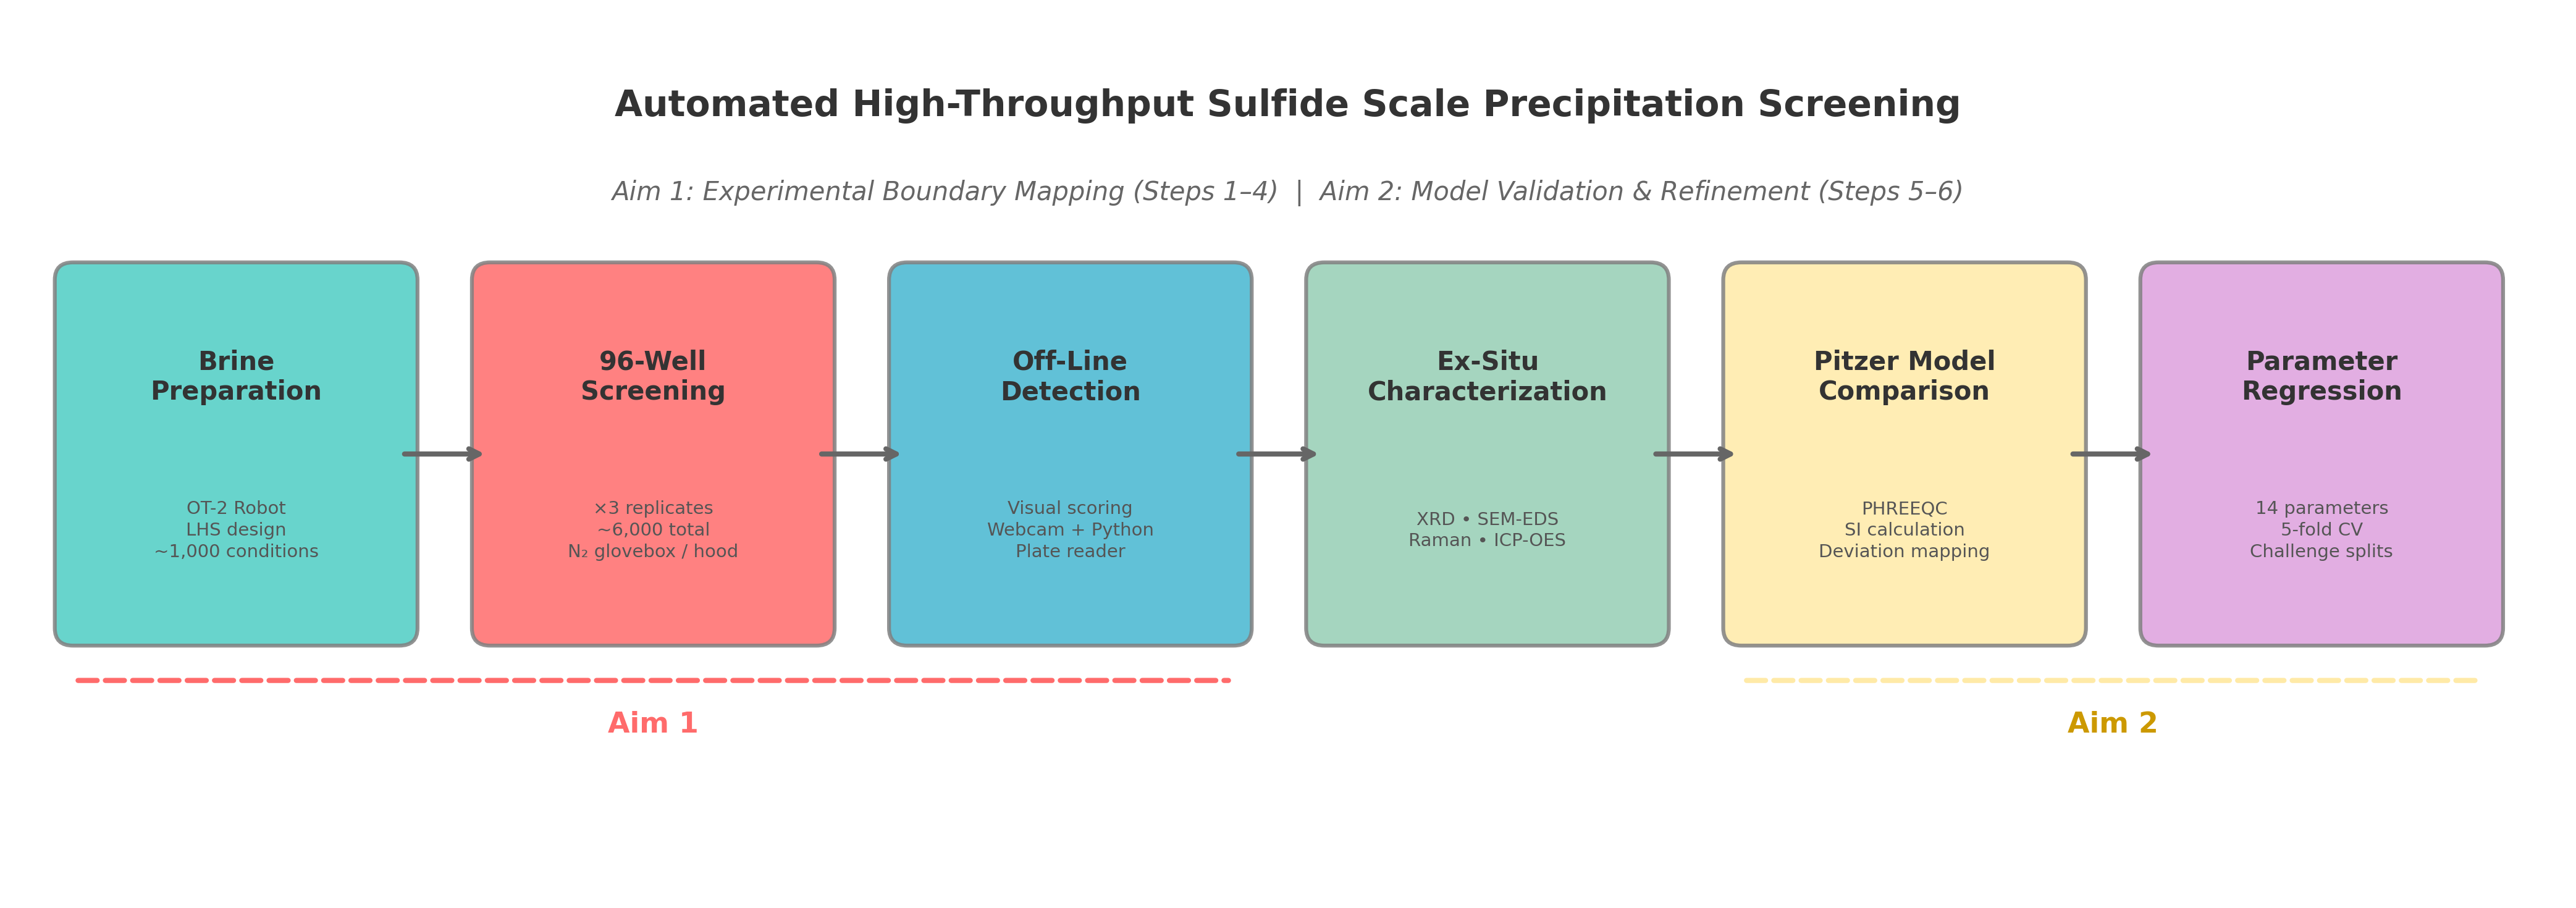
\includegraphics[width=0.35\textwidth]{../grants/acs-prf/figures/workflow-diagrams/experimental_workflow.png}
\caption{Aim~1 workflow. The high-throughput experimental platform dispenses stock solutions of metal salts, Na$_2$S/NaHS, NaCl, CaCl$_2$, and pH buffers into 96-well plates according to a Latin hypercube sampling design. Plates are then transferred to an off-line detection station (visual scoring, camera imaging, or microplate reader) to identify precipitation vs.\ no-precipitation for each condition.}
\label{fig:aim1}
\vspace{-1em}
\end{wrapfigure}

\textbf{Stock solution preparation.} Concentrated stock solutions of FeSO$_4$ (or FeCl$_2$), PbCl$_2$, Na$_2$S$\cdot$9H$_2$O (or NaHS), NaCl, CaCl$_2$, and pH buffer components (acetate, MES, HEPES, and bicarbonate) will be prepared gravimetrically in deoxygenated ultrapure water. For iron(II) experiments, all Fe$^{2+}$-containing solutions will be prepared and dispensed inside a standard N$_2$ glovebox to prevent oxidation to Fe(III); critically, the OT-2 will be placed \textit{inside} the glovebox for Fe$^{2+}$ campaigns, because standard 96-well plates are not gas-tight and even trace O$_2$ can produce confounding iron oxyhydroxide precipitates within hours \cite{wang2024}. A general-purpose inert-atmosphere glovebox (N$_2$, with continuous O$_2$ monitoring) is sufficient; the ultradry ($<$1~ppm H$_2$O) conditions required for battery or air-sensitive organometallic work are \textit{not} needed, since all solutions are aqueous. The glovebox will therefore not be compromised for more moisture-sensitive projects. Pb$^{2+}$ experiments do not require inert atmosphere and will be conducted in the fume hood.

\textbf{Experimental design.} Rather than a conventional full factorial grid, we will employ a Latin hypercube sampling (LHS) design \cite{mckay1979} to efficiently fill the five-dimensional parameter space (metal-ion concentration, sulfide concentration, ionic strength, pH, and temperature) with near-uniform coverage while requiring fewer total experiments than a full factorial. LHS ensures that projections onto each individual variable axis are evenly sampled, which is critical for subsequent regression of Pitzer parameters that may depend differently on each variable. For each metal system (Fe$^{2+}$, Pb$^{2+}$), we will generate approximately 2,500 unique LHS conditions spanning: metal-ion concentration (0.01--100~mM, log-spaced), sulfide concentration (0.01--50~mM, log-spaced), ionic strength (0.5--5~molal NaCl $\pm$ 0.5~molal CaCl$_2$), pH (4--9), and temperature (25, 60, 90~$^\circ$C). Each 96-well plate will contain a unique set of LHS-sampled conditions plus matrix-matched blanks and BaSO$_4$ positive controls. Three replicate plates will be prepared for each batch of conditions to enable statistical uncertainty quantification, yielding approximately 7,500 initial measurements per metal system ($\sim$15,000 total across both systems). An additional $\sim$15,000 measurements will be generated via BO-guided follow-up (see below), bringing the grand total to approximately 30,000 experiments. All experimental metadata---timestamps, ambient temperature, humidity, solution ages, and OT-2 protocol version---will be recorded in a structured database to support reproducibility and future reanalysis.

\textbf{Adaptive follow-up via Bayesian optimization.} After the initial LHS campaign identifies the approximate precipitation boundaries, we will employ high-dimensional Bayesian optimization (BO) to adaptively select follow-up conditions that maximally constrain the 34 Pitzer parameters. Bayesian optimization constructs a probabilistic surrogate model of the objective function and uses an acquisition function to select the next experiment that is most informative---concentrating sampling near the precipitation boundary where parameter sensitivity is highest. The high parameter dimensionality (34) is well within the demonstrated capabilities of modern BO algorithms: Baird et al.\ (2022) demonstrated the effectiveness of the SAASBO (Sparse Axis-Aligned Subspace Bayesian Optimization) algorithm for optimizing 23 parameters simultaneously \cite{baird2022,eriksson2021}, which is directly applicable to the 34-parameter space of this project. A key advantage of BO for this application is its \textit{rich interpretability}: the trained surrogate model provides uncertainty estimates across the entire parameter space, reveals which experimental variables most influence precipitation boundaries, and enables sensitivity analysis of individual Pitzer parameters. If practical delays arise in implementing BO---for example, due to high experimental noise that challenges surrogate modeling---we can fall back to additional quasi-random (Sobol or Halton) sampling points to augment the dataset without requiring model-guided decisions. This hybrid LHS$+$BO strategy ensures both broad coverage and targeted refinement of the precipitation boundary.

\textbf{High-throughput sample preparation.} An Opentrons OT-2 robot equipped with single-channel and 8-channel pipettes (GEN2, 20--300~$\mu$L) will dispense stock solutions into 96-well plates. The 8-channel pipette enables rapid row-wise dispensing of matrix solutions (NaCl, CaCl$_2$, buffer), while the single-channel pipette delivers metal and sulfide stock solutions at condition-specific volumes. Mixing will be achieved by repeated aspiration/dispense cycles. The robot's Python API enables scripted, reproducible protocols with full logging of volumes, well positions, and timestamps.

\textbf{Detection.} After robotic plate preparation, precipitation will be detected \textit{off-line} (no custom OT-2 module required) by three complementary methods of increasing sophistication: (1)~\textit{Visual binary scoring}: both FeS (black) and PbS (black/brown) precipitates are readily visible against the clear background of a well plate. A researcher scores each well as precipitate/no-precipitate, providing the binary outcome required for Aim~2. This baseline approach ensures meaningful data collection even without specialized instruments. (2)~\textit{Camera imaging}: a camera mounted above the plate captures images at defined time points, and automated Python image analysis classifies wells as clear, turbid, or colored based on RGB/grayscale thresholds. This low-cost method ($<$\$100 in hardware) provides semi-quantitative, time-resolved data. (3)~\textit{Microplate-reader absorbance/turbidity}: absorbance at 600~nm or forward-scatter provides quantitative turbidity measurements for precise precipitation-onset determination. During the initial project months (1--6), we will use visual scoring and camera imaging to establish the workflow and begin data collection; these approaches alone yield the binary precipitation/no-precipitation data required for Aim~2. Microplate-reader measurements will be obtained through BYU's shared-instrumentation facilities (the College of Engineering maintains multi-mode plate readers such as the BioTek Synergy H1 or Molecular Devices SpectraMax iD3); if shared-instrument scheduling proves limiting, a dedicated reader can be procured from the PI's startup or equipment funds at no cost to this grant. Time-resolved measurements (at 1, 5, 15, 60, and 240~minutes post-mixing) will distinguish rapid thermodynamic precipitation from slow kinetic nucleation. A subset of $\sim$100 conditions near the predicted precipitation boundary will be equilibrated for 24--72~hours in sealed glass vials to verify that the 240-minute endpoint approximates thermodynamic equilibrium; where kinetic delays are observed, the longer-equilibration data will take precedence for parameter regression. Critically, the OT-2 automates the most labor-intensive step---preparing hundreds of unique brine compositions reproducibly---while detection requires only transferring the plate to a reader or camera station, a workflow compatible with a single researcher.

\textbf{Controls and quality assurance.} Each plate will include matrix-matched blanks (no metal or no sulfide) to establish baseline turbidity in high-TDS solutions. Positive controls using BaSO$_4$ precipitation (well-characterized thermodynamics) will validate the detection methodology at each ionic strength. Chemically resistant, optically clear polypropylene or polystyrene 96-well microplates will be used to enable both absorbance/imaging measurements and compatibility with sulfide solutions. Adhesive plate seals will be applied immediately after dispensing to minimize H$_2$S off-gassing and evaporation during time-course measurements. Cross-contamination will be prevented by using disposable, filter-tipped pipette tips for every aspiration/dispense step---a standard practice with the OT-2 that is scripted into the protocol. For \textit{human-in-the-loop validation}, a subset of 50--100 conditions showing precipitation near the boundary will be repeated manually at larger scale (5~mL vials) with gravimetric or ICP-OES confirmation of dissolved metal concentrations. At the end of each experimental campaign, an \textit{end-of-campaign validation study} will compare a randomly selected set of 20--30 conditions against independent manual preparations to verify inter-method reproducibility.

\subsection{Aim 2: Pitzer-Model Comparison and Parameter Regression}

\begin{wrapfigure}{r}{0.4\textwidth}
\centering
\vspace{-1.5em}
\fbox{\rule{0pt}{1.5in}\rule{0.35\textwidth}{0pt}}
\caption{Aim~2 analysis pipeline. Experimental precipitation boundaries are compared to Pitzer-model predictions (via PHREEQC) to generate deviation maps across the parameter space. Where deviations exceed $\pm$0.2~SI, new Pitzer interaction parameters are regressed and validated against held-out data.}
\label{fig:aim2}
\vspace{-1em}
\end{wrapfigure}

\textbf{Thermodynamic modeling.} For each experimental condition, we will calculate the saturation index (SI~$= \log(Q/K_{\text{sp}})$) using PHREEQC with the Pitzer database (pitzer.dat) and, where available, supplementary interaction parameters from the recent literature \cite{kan2019,wang2020,felmy2000}. The speciation calculation will explicitly account for metal--chloride complexation (e.g., FeCl$^+$, PbCl$^+$, PbCl$_2^0$, PbCl$_3^-$), metal--sulfide complexation (e.g., FeHS$^+$, FeS$^0_{\text{aq}}$), sulfide protonation equilibria (H$_2$S/HS$^-$/S$^{2-}$), and ion-pair formation---ensuring that missing Pitzer parameters are not artificially compensated by neglecting speciation \cite{felmy2000}. Wang (2024) demonstrated that fitting Pitzer coefficients for Fe--HS, Fe--Cl, and Fe--SO$_4$ pairs simultaneously---including the FeS$^0_{\text{aq}}$ stability constant---yields a mean SI error of $\pm$0.015 across 154 data points spanning 0--5~mol/kg ionic strength and 23--125~$^\circ$C \cite{wang2024}; we will adopt Wang's Fe$^{2+}$--HS$^-$ binary parameters as initial values and benchmark the Fe system against this framework and PHREEQC's \texttt{pitzer.dat}. For Fe$^{2+}$--Cl$^-$ interactions and for the Pb system more broadly, we will additionally compare to Bozau's gebo database \cite{bozau2013}, noting that Fe$^{2+}$--HS$^-$ binary Pitzer parameters are not documented in gebo and are therefore a primary target of regression in this work. Of the 34 target parameters, 3 (Fe$^{2+}$--HS$^-$ binary) have preliminary estimates from Wang (2024) and 3 (Pb$^{2+}$--Cl$^-$ temperature-dependent) from Woosley \& Millero (2013) \cite{woosley2013}, requiring independent validation; the remaining 28 have no prior estimates in any database. The specific supplementary parameters to be evaluated and, where necessary, re-determined include: 6 binary parameters ($\beta^{(0)}$, $\beta^{(1)}$, $C^\phi$) for Fe$^{2+}$--HS$^-$ and Pb$^{2+}$--HS$^-$ (3 per metal system); 8 higher-order mixing parameters---$\theta_{\text{Fe--Na}}$, $\theta_{\text{Fe--Ca}}$, $\theta_{\text{Pb--Na}}$, $\theta_{\text{Pb--Ca}}$, $\psi_{\text{Fe--Na--Cl}}$, $\psi_{\text{Fe--Ca--Cl}}$, $\psi_{\text{Pb--Na--Cl}}$, and $\psi_{\text{Pb--Ca--Cl}}$; neutral-species interaction parameters for FeS$^0_{\text{aq}}$ and PbS$^0_{\text{aq}}$---$\lambda_{\text{n,Na}}$, $\lambda_{\text{n,Cl}}$, $\zeta_{\text{n,Na,Cl}}$, and $\zeta_{\text{n,Ca,Cl}}$ for each complex (8 total); temperature-dependent Pb$^{2+}$--Cl$^-$ coefficients (3 parameters); metal--hydroxide interaction corrections at elevated pH (2 parameters); Pb$^{2+}$--SO$_4^{2-}$ binary parameters ($\beta^{(0)}$, $\beta^{(1)}$, $C^\phi$; 3 parameters), required because produced-water brines routinely contain sulfate alongside sulfide \cite{felmy2000,kan2019}; and neutral-species interaction parameters for PbCl$_2^0$ ($\lambda_{\text{n,Na}}$, $\lambda_{\text{n,Cl}}$, $\zeta_{\text{n,Na,Cl}}$, $\zeta_{\text{n,Ca,Cl}}$; 4 parameters), needed because Pb$^{2+}$ forms significant chloro-complexes in high-chloride brines \cite{mgaidi1991}---for a total of 34 parameters across the two metal systems.

Preliminary PHREEQC calculations confirm the scope of this gap (Figure~\ref{fig:phreeqc_si}). When saturation indices for BaSO$_4$, FeS (mackinawite), and PbS (galena) are computed across 0.1--5.0~molal NaCl at 25~$^\circ$C, the BaSO$_4$ Pitzer model shows a 1.3~SI-unit response to ionic strength, reflecting the well-parameterized Ba$^{2+}$--Na$^+$--Cl$^-$ interactions. In contrast, the FeS and PbS curves---computed with the Davies equation because no Pitzer parameters exist---vary by only 0.1 and 0.8~SI units, respectively. Galena is not even defined as a phase in the standard PHREEQC databases. These flat Davies-equation curves are unreliable above $I \approx 0.5$~molal and cannot capture the specific ion--ion interactions that govern precipitation in produced-water brines.

\begin{figure}[htbp]
\centering
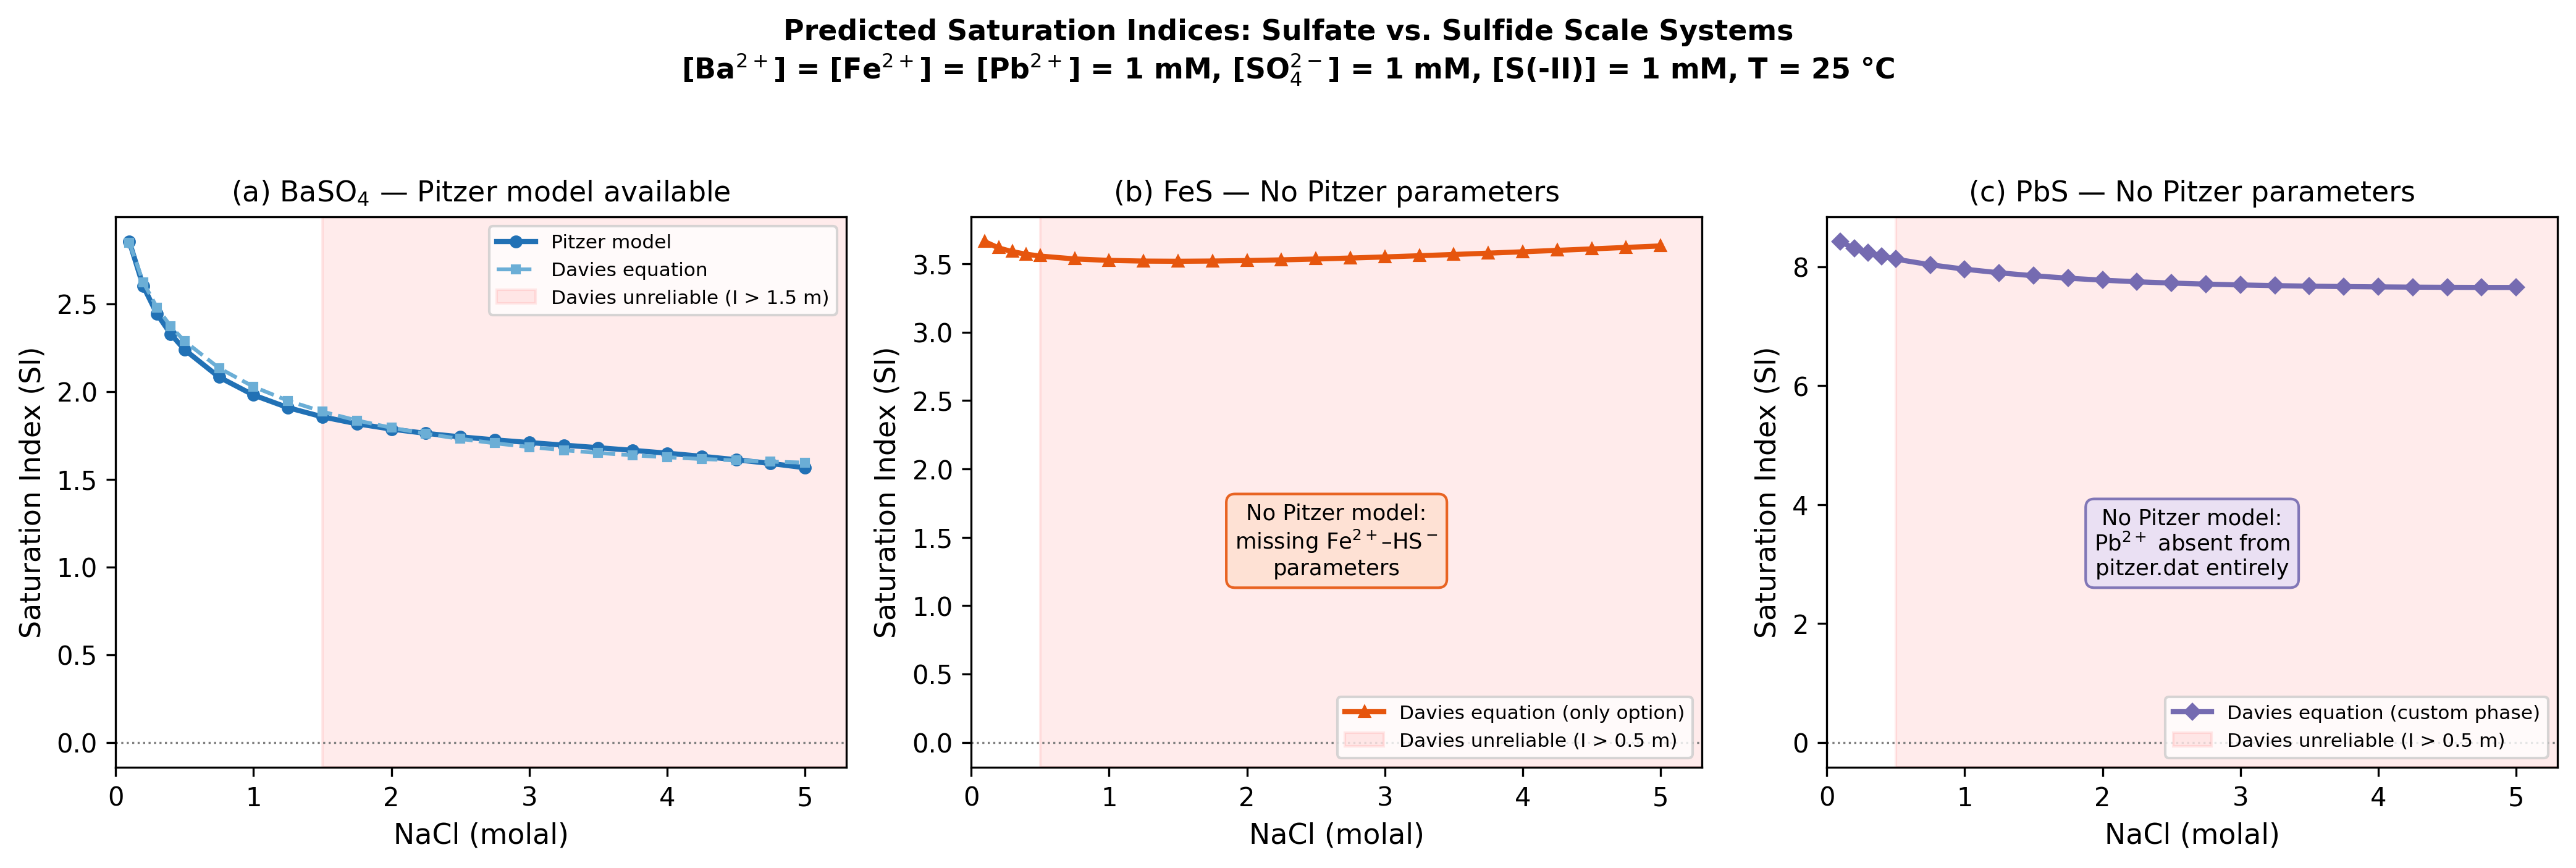
\includegraphics[width=\textwidth]{../preliminary_results/phreeqc_si_comparison.png}
\caption{Predicted saturation indices as a function of NaCl concentration (0.1--5.0~molal) at 25~$^\circ$C for (a)~BaSO$_4$ using the Pitzer model (validated parameters available), (b)~FeS using only the Davies equation (no Fe$^{2+}$--HS$^-$ Pitzer parameters exist), and (c)~PbS using the Davies equation with a custom Galena phase definition (Pb$^{2+}$ is entirely absent from \texttt{pitzer.dat}). The flat sulfide curves at high ionic strength reflect the known limitation of the Davies equation above $I \approx 0.5$~molal. \textbf{This gap is the target of the proposed research.}}
\label{fig:phreeqc_si}
\end{figure}

\textbf{Comparison framework.} The binary experimental outcome (precipitation observed vs.\ not observed) at each condition defines an empirical precipitation boundary. This boundary will be compared to the model-predicted SI~$= 0$ contour. Systematic offsets---such as the model predicting SI~$> 0$ (supersaturation and expected precipitation) at conditions where no precipitate is observed---will indicate that the model overestimates the effective ion activities, implicating missing or inaccurate interaction parameters.

\textbf{Image analysis pipeline.} All plate images (camera) will be archived in a structured repository with associated metadata, enabling retrospective reanalysis. During the initial phase, precipitation calls will be made by \textit{manual annotation}---a researcher labels each well as clear or precipitated---providing a reliable ground-truth dataset. As the annotated image library grows (anticipated $>$2,000 labeled wells within the first campaign), we will develop a simple computer-vision classifier as a \textit{stretch goal}. Thresholding on grayscale intensity or color-channel ratios (OpenCV; \cite{bradski2000}) provides a natural starting point for black FeS/PbS precipitates against a clear background; if needed, a lightweight convolutional neural network can be trained on the accumulated manual labels. This phased approach ensures that the core science (Aim~2) proceeds on manually validated data while building toward automated image classification that would accelerate future campaigns.

\textbf{Parameter regression.} Where the average deviation between predicted and observed boundaries exceeds $\pm$0.2~SI, we will regress the full set of 34 parameters using weighted nonlinear least-squares optimization with ridge regularization to mitigate parameter correlations (particularly between $\beta^{(0)}$ and $C^\phi$); model complexity will be assessed via the Bayesian Information Criterion (BIC) to determine the minimum parameter set justified by the data. The mixing parameters include: (1)~$\theta_{\text{Fe--Na}}$ and $\psi_{\text{Fe--Na--Cl}}$ for FeS in NaCl brines; (2)~$\theta_{\text{Fe--Ca}}$ and $\psi_{\text{Fe--Ca--Cl}}$ for FeS in CaCl$_2$-bearing brines; (3)~$\theta_{\text{Pb--Na}}$ and $\psi_{\text{Pb--Na--Cl}}$ for PbS in NaCl brines; (4)~$\theta_{\text{Pb--Ca}}$ and $\psi_{\text{Pb--Ca--Cl}}$ for PbS in CaCl$_2$-bearing brines; plus binary, neutral-species, and temperature-dependent terms as enumerated above. Initial values will be drawn from Pitzer's combining rules as starting points. As a core component of the parameter regression, $\sim$200--300 conditions spanning the ionic-strength range will be selected for quantitative dissolved-metal analysis via ICP-OES, providing continuous concentration data essential for constraining individual Pitzer parameters that are correlated along the saturation-index surface. Binary precipitation data alone constrain only the SI~$= 0$ contour; continuous dissolved-metal concentrations provide information about the magnitude of supersaturation and are therefore critical for resolving parameter correlations.

\textbf{Validation.} The regressed parameters will be validated by predicting precipitation boundaries for a set of held-out experimental conditions (20\% of the dataset, randomly selected before fitting) and for literature data where available. We will employ 5-fold cross-validation---a standard technique in which the dataset is partitioned into five equal subsets, the model is trained on four subsets and tested on the fifth, and the process is repeated for each subset to yield an unbiased estimate of predictive accuracy \cite{arlot2010}. To assess extrapolatory performance, we will additionally construct ``challenge'' splits in which all data above a specific ionic-strength threshold (e.g., $I > 3$~molal) are withheld during fitting; predictive accuracy on these held-out high-$I$ conditions will reveal whether the regressed parameters generalize beyond the training domain. A successful outcome is defined as reducing the average SI deviation to $< \pm$0.1~SI across the full parameter space.

\subsection{Timeline}

\textbf{Year~1} (Months 1--12): Stock solution preparation and protocol validation (Months 1--3); FeS precipitation boundary mapping at 25~$^\circ$C across ionic strength and pH (Student~1, Months 3--10) conducted in parallel with Pb$^{2+}$ precipitation mapping at 25~$^\circ$C (Student~2, Months 3--10); begin PHREEQC modeling and Bayesian optimization--guided follow-up experiments (Months 8--12). \textbf{Year~2} (Months 13--24): Temperature-dependent measurements for both systems (Months 13--18); BO-guided adaptive sampling near identified precipitation boundaries (Months 13--18); concurrent with data collection, complete Pitzer-model comparisons and parameter regression (Months 15--21); manuscript preparation and submission (Months 18--24).

\textbf{Fitting strategy.} We will adopt a hierarchical fitting approach as the primary regression strategy: first fix Pb$^{2+}$--Cl$^-$ and Pb$^{2+}$--SO$_4^{2-}$ parameters at published values \cite{felmy2000,woosley2013,mgaidi1991} and adopt Wang's (2024) Fe$^{2+}$--HS$^-$ binary coefficients as initial values \cite{wang2024}, reducing the initial free parameter count to $\sim$22; sulfide-specific mixing and neutral-species terms will be regressed first, and additional parameters released sequentially as the dataset grows and parameter identifiability improves. If Fe$^{2+}$ oxidation proves difficult to control despite glovebox preparation, we will prioritize the PbS system (which requires no inert atmosphere) and treat FeS as a secondary campaign once the oxidation-control protocol is validated, reducing the active parameter set to $\sim$17. If shared microplate-reader access is insufficient for the required throughput, the visual-scoring and camera-imaging tiers alone provide the binary data needed for parameter regression (Aim~2), and the PI's startup funds can support procurement of a dedicated reader if needed. If the LHS design reveals unexpected clustering of conditions near phase boundaries, we will supplement with targeted BO-guided or quasi-random follow-up plates in those regions. If high experimental noise or other practical difficulties impede the Bayesian optimization surrogate model, we will revert to additional quasi-random (Sobol or Halton) sampling points to augment the dataset without requiring model-guided decisions.

\section{Expected Results and Impact}

We expect that existing Pitzer models will accurately predict FeS and PbS precipitation at low ionic strengths ($I < 1$~molal) but will systematically deviate at ionic strengths above $\sim$2~molal, which are typical of petroleum-produced waters. This expectation is grounded in the mathematical structure of the Pitzer equations: at low $I$, the Debye--H\"uckel term dominates and binary parameters suffice, but at high $I$ the higher-order mixing terms ($\theta_{ij}$, $\psi_{ijk}$) become significant. Because these terms are absent for sulfide systems, the model extrapolates without the corrections that have been shown essential for sulfate scales \cite{kan2019}. The Pb$^{2+}$ system represents the most severe gap: Felmy et al.\ (2000) showed that even chloride--sulfate models for Pb$^{2+}$ fail above $I \approx 2$~molal \cite{felmy2000}, and no sulfide interactions have been parameterized at all. For FeS, additional complexity arises from metastable precursor phases and nanoparticulate intermediates that may not conform to macroscopic equilibrium predictions \cite{kan2019}; our experimental design addresses this by measuring precipitation onset rather than equilibrium solubility, and by comparing to multiple proposed $K_{\text{sp}}$ values. Specifically, we anticipate that the models will overpredict supersaturation---predicting precipitation at conditions where the brine remains undersaturated---because unmeasured repulsive interactions between scale-forming cations (Fe$^{2+}$, Pb$^{2+}$) and abundant matrix cations (Na$^+$, Ca$^{2+}$) effectively increase sulfide-mineral solubility beyond what current parameters capture.

The largest deviations for FeS are expected at near-neutral pH (6--7.5) in Ca$^{2+}$-rich brines, where Ca$^{2+}$--Fe$^{2+}$ interactions and CaHS$^+$ complexation are most significant but least constrained. For PbS, deviations are expected to increase with temperature (60--90~$^\circ$C) and NaCl concentration, where Pb$^{2+}$--Cl$^-$ complexation competes with Pb$^{2+}$--HS$^-$ interactions. If these predictions are confirmed, the new Pitzer interaction parameters will provide a quantitative resolution. If the existing parameters prove adequate across the full range (deviations $< \pm$0.2~SI), this itself would be a significant finding, indicating that the current thermodynamic database is more robust than the literature suggests.

The broader impact of this work is threefold. First, the validated Pitzer parameters will be directly usable by the petroleum engineering community to improve sulfide-scale prediction in produced-water management. Second, the automated high-throughput precipitation screening methodology will be transferable to other mineral-scale systems, including CaCO$_3$ and SrSO$_4$. Third, this project will generate preliminary data for a larger proposal (NSF CAREER or CHE) to extend the Pitzer database to additional scale-forming minerals and to develop predictive models for mixed-scale precipitation in complex brines.

\section{Student Training Plan}

This project will support two master's-level graduate students and two part-time undergraduate researchers over the two-year grant period. BYU's Department of Mechanical Engineering enrolls a large M.S.\ cohort, and master's students regularly complete thesis-based research within 2~years---well-matched to the ACS PRF timeline. The M.S.\ students will begin in Year~1 and will conduct FeS and PbS precipitation experiments, PHREEQC thermodynamic modeling, and Pitzer parameter regression in parallel. The students will receive training in four key areas: (1)~\textit{inorganic aqueous chemistry}, including solution thermodynamics, activity-coefficient models, and metal-ion speciation; (2)~\textit{automated experimentation}, including robotic sample preparation (Python/Opentrons API), experimental design, and high-throughput data collection; (3)~\textit{computational modeling}, including PHREEQC thermodynamic calculations, nonlinear parameter regression, and data visualization; and (4)~\textit{scientific communication}, including thesis writing, conference presentations, and data management. Students will be encouraged to take elective courses across BYU departments to strengthen their interdisciplinary preparation, including CHEM~561 (Chemical Thermodynamics), CHEM~521 (Instrumental Analysis), ME~EN~575 (Optimization Techniques in Engineering), and STAT~536 (Statistical Learning and Data Mining).

Undergraduate researchers will contribute to stock solution preparation, data collection, and image analysis during the academic year and summer. BYU has a strong culture of undergraduate research participation, and these positions will provide hands-on experience with quantitative inorganic chemistry techniques and exposure to modern research methods including robotic laboratory automation and computational thermodynamics---competencies increasingly valued in industrial and academic careers. All students will present their work at ACS national or regional meetings and will be co-authors on resulting publications.

\todo[inline]{Add text noting that, given the PI's newness to aqueous geochemistry and sulfide chemistry, [name of collaborator/mentor] has expressed support to informally mentor the PI on this project. Identify a BYU or external colleague with aqueous geochemistry or oilfield chemistry expertise (e.g., from the Chemistry or Geological Sciences departments).}

%TC:ignore
\vspace{1em}
\noindent\textit{Word count (body text, excluding abstract, captions, and references): \wordcount{} / 4{,}000}
%TC:endignore

% \section{References}

\begin{singlespace}
\bibliographystyle{unsrtnat}
\bibliography{references}
\end{singlespace}

\end{document}
